\documentclass{article}

\usepackage{graphicx}
\usepackage{tikz}
\usepackage{tikzsymbols}
\usetikzlibrary{calc,patterns,shapes.geometric}
\pagestyle{empty}
\usepackage[margin=0pt]{geometry}
\geometry{papersize={14in,12in}}

\def\centerarc[#1](#2)(#3:#4:#5){\draw[#1] ($(#2)+({#5*cos(#3)},{#5*sin(#3)})$) arc (#3:#4:#5);}

\begin{document}
	\begin{figure}
		\centering
		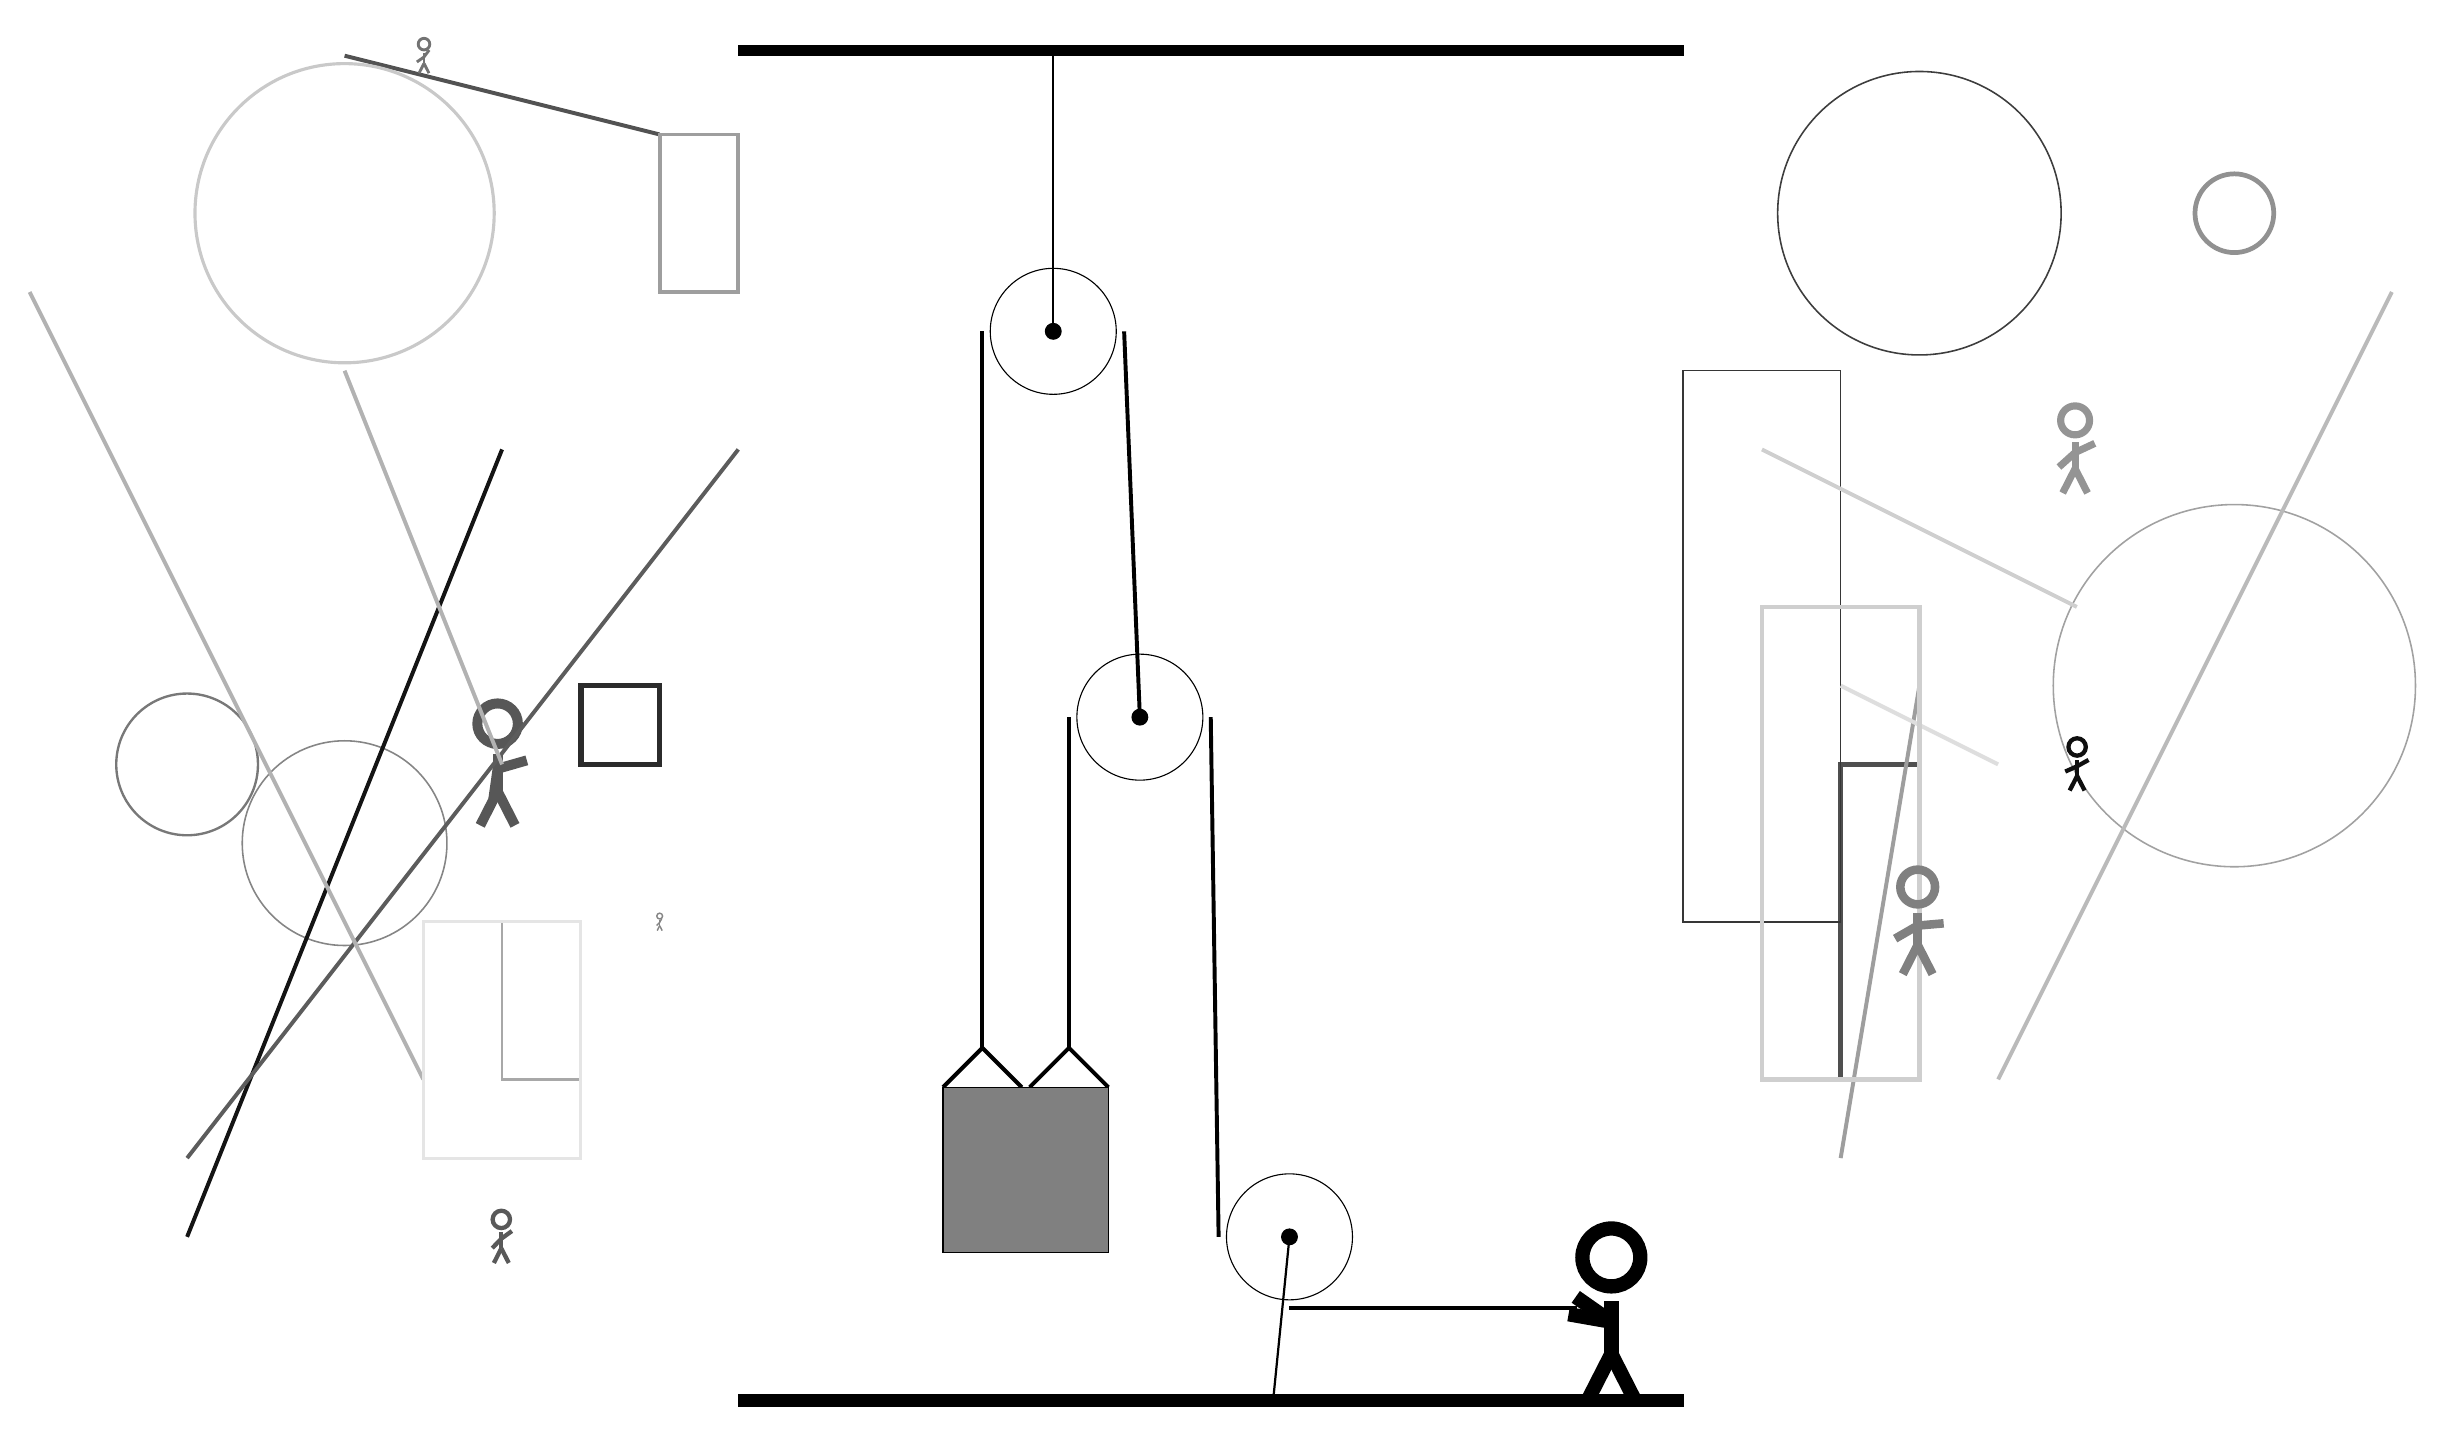
\begin{tikzpicture}
			%%%%% START %%%%%
			
			\draw[fill=black] (-2, 14) rectangle (10, 14.125);
			
			\draw (2, 10.5) circle (0.8);
			\draw[fill=black] (2, 10.5) circle (0.1);
			\draw[thick] (2, 10.5) -- (2, 14);
			
			\draw (3.1, 5.6) circle (0.8);
			\draw[fill=black] (3.1, 5.6) circle (0.1);
			
			\draw [line width=0.6mm, color=black!43](17, 12) circle (0.5);
			
			\draw [line width=0.2mm, color=black!37](17, 6) circle (2.3);
			\node[line width=0.3mm, color=black!94] at (15, 5) {\Strichmaxerl[3][24][29]};
			\draw [line width=0.2mm, color=black!48](-7, 4) circle (1.3);
			\draw[line width=0.6mm, color=black!69] (12, 5) rectangle (13, 1);
			\draw[line width=0.5mm, color=black!68](-3, 13) -- (-7, 14);
			\draw [line width=0.3mm, color=black!53](-9, 5) circle (0.9);
			\draw[line width=0.5mm, color=black!92](-5, 9) -- (-9, -1);
			\draw[line width=0.5mm, color=black!38](13, 6) -- (12, 0);
			
			\draw[line width=0.2mm, color=black!79] (10, 10) rectangle (12, 3);
			\draw [line width=0.2mm, color=black!91](11, 10) circle (0.0);
			\draw[line width=0.5mm, color=black!19](11, 9) -- (15, 7);
			\node[line width=0.5mm, color=black!66] at (-5, 5) {\Strichmaxerl[7][82][16]};
			
			\draw[line width=0.5mm, color=black!13](14, 5) -- (12, 6);
			\draw [line width=0.2mm, color=black!76](13, 12) circle (1.8);
			\draw[line width=0.6mm, color=black!19] (11, 7) rectangle (13, 1);
			
			\draw [line width=0.4mm, color=black!21](-7, 12) circle (1.9);
			\node[line width=0.7mm, color=black!65] at (-5, -1) {\Strichmaxerl[3][46][36]};
			\node[line width=0.7mm, color=black!55] at (-6, 14) {\Strichmaxerl[2][35][53]};
			
			\draw[line width=0.5mm, color=black!64](-2, 9) -- (-9, 0);
			\draw[line width=0.5mm, color=black!30](-6, 1) -- (-11, 11);
			
			\draw[line width=0.5mm, color=black!30](-5, 5) -- (-7, 10);
			
			\draw[line width=0.3mm, color=black!34] (-4, 3) rectangle (-5, 1);
			\node[line width=0.3mm, color=black!50] at (13, 3) {\Strichmaxerl[6][30][5]};
			\draw[line width=0.7mm, color=black!83] (-4, 6) rectangle (-3, 5);
			
			\draw[line width=0.4mm, color=black!10] (-4, 3) rectangle (-6, 0);
			
			\node[line width=0.4mm, color=black!48] at (-3, 3) {\Strichmaxerl[1][44][63]};
			\draw[line width=0.5mm, color=black!38] (-2, 11) rectangle (-3, 13);
			
			\node[line width=0.4mm, color=black!42] at (15, 9) {\Strichmaxerl[5][42][25]};
			\draw[line width=0.5mm, color=black!27](14, 1) -- (19, 11);
			
			\draw (5, -1) circle (0.8);
			\draw[fill=black] (5, -1) circle (0.1);
			\draw[thick] (5, -1) -- (4.8, -3);
			
			\draw[line width = 0.5mm]  (0.6, 0.9) -- (1.1, 1.4) -- (1.6, 0.9);
			\draw[line width = 0.5mm]  (1.7, 0.9) -- (2.2, 1.4) -- (2.7, 0.9);
			\draw[fill=black!50] (0.6, 0.9) rectangle (2.7, -1.2);
			
			\draw[line width = 0.5mm] (1.1, 10.5) -- (1.1, 1.4);
			\centerarc[line width = 0.5mm](2, 10.5)(0:180:0.9);
			\draw[line width = 0.5mm] (2.9, 10.5) -- (3.1, 5.6);
			\draw[line width = 0.5mm] (2.2, 5.6) -- (2.2, 1.4);
			\centerarc[line width = 0.5mm](3.1, 5.6)(0:180:0.9);
			\draw[line width = 0.5mm] (4.0, 5.6) -- (4.1, -1);
			\centerarc[line width = 0.5mm](5, -1)(180:270:0.9);
			\draw[line width = 0.5mm] (5, -1.9) -- (8.65, -1.9);
			
			\node at (9, -2) {\Strichmaxerl[10][-35][170]};
			
			\draw[fill=black] (-2, -3) rectangle (10, -3.15);
			
			%%%%% END %%%%%
		\end{tikzpicture}
	\end{figure}	
\end{document}